% Präabel ====================================================================
\documentclass[12pt,a4paper,oneside]{article}
% PDF-Version 1.7 verwenden anstatt der 15 Jahre alten 1.5 (sorgt auch für weniger Warnungen, da die meisten PDF-Bilder mittlerweile Version 1.7 sind.)
% Ich weiß nicht, wieso PDFTeX immer noch per default 1.5 verwendet.

		
\pdfminorversion=7
\usepackage[a4paper]{geometry}
% Seitenrahmen 
\geometry{a4paper,left=20mm,right=20mm,bottom=20mm,top=15mm}
%passende Codierung
\usepackage[utf8]{inputenc}
% Umlaute Version 
\usepackage[english]{babel}
\usepackage[T1]{fontenc}
\usepackage{lmodern}
\usepackage[german=quotes]{csquotes}
% Mathe-Package
\usepackage{amsmath}
% Mathesymbole
\usepackage{amssymb}
\usepackage{mathtools}
\usepackage{amsthm}
%Grafiken einfügen, .pdf einfügen, grafiken in Unterordner festlegen
\usepackage[pdftex]{graphicx}
\usepackage{pdfpages}
\graphicspath{{git_graphics/}}
\usepackage{tabularx}
\usepackage{float}
\usepackage{setspace}
\onehalfspacing
%% Unused
%\usepackage{tikz}
%\usetikzlibrary{shapes,arrows}
\usepackage{trfsigns}
\usepackage{hyperref}
\usepackage{calc}

\usepackage{titlesec}
\titleformat{\paragraph}
{\normalfont\normalsize\bfseries}{\theparagraph}{1em}{}
\titlespacing*{\paragraph}
{0pt}{3.25ex plus 1ex minus .2ex}{1.5ex plus .2ex}
\setcounter{secnumdepth}{5}
\setcounter{tocdepth}{5}

\usepackage{xcolor} 

%\usepackage[backend=biber,style=IEEE]{biblatex}
\usepackage[bibstyle=ieee]{biblatex}
\addbibresource{bibliography.bib}


\usepackage{listings}
\definecolor{hellgelb}{rgb}{1,1,0.9}
\definecolor{quellcode_comment}{rgb}{0.2,0.6,0.2}
\definecolor{quellcode_string}{rgb}{0.6,0,0.8}
\definecolor{quellcode_background}{rgb}{0.98,0.98,0.98}

\lstset{numbers=left,
				backgroundcolor=\color{hellgelb},
				breaklines=true,
				frame=single,
				captionpos=b,
 				language=Matlab,
 				basicstyle=\ttfamily\color{black}\scriptsize,
 				keywordstyle=\color{blue},
 				commentstyle=\color{quellcode_comment},
 				stringstyle=\color{quellcode_string}
				}
\renewcommand{\lstlistingname}{Code} 


%% Überschreibungen
% set imaginary unit to j
\renewcommand{\j}{\mathrm{j}}
% Untertilde
\newcommand{\utilde}[1]{\underset{\sim}{#1}}
% Vektor fett und unterstrichen
\renewcommand{\vec}[1]{\ensuremath{\underline{\boldsymbol {#1}}}}	
% Vektor fett und unterstrichen
\newcommand{\vecp}[1]{\ensuremath{\overrightarrow{\boldsymbol {#1}}}}	
% Dicker Ableitungspunkt
\renewcommand*{\dot}[1]{\accentset{\mbox{\textrm{\large\bfseries .}} }{#1}}						
% Dicker Doppelableitungspunkt
\renewcommand*{\ddot}[1]{\accentset{\mbox{\textrm{\large\bfseries .\hspace{-0.25ex}.}}}{#1}}	
% Dicker Dreifachableitungspunkt
\renewcommand*{\dddot}[1]{\accentset{\mbox{$\overset{\textrm{\large\bfseries .}}{\textrm{\large\bfseries.\hspace{-0.25ex}.}}$}}{#1}}	
% Definiere  Matrizen
\newcommand{\ma}[1]{\ensuremath{\utilde{\boldsymbol {#1}}}}			% Matrixsymbol
\newcommand{\mat}[1]{\ensuremath{\begin{bmatrix} #1 \end{bmatrix}}}	% Matrix
% Real und Imaginärteil
\renewcommand{\Re}[1]{\ensuremath{\operatorname{Re}\left\{#1\right\}}}
\renewcommand{\Im}[1]{\ensuremath{\operatorname{Im}\left\{#1\right\}}}

\newcommand{\textcirc}[1]{\textrm{\textcircled{#1}}}

\newcommand{\abs}[1]{\ensuremath{\left| #1 \right|}}

% Abkürzungen für Symbole
\providecommand{\ul}[1]{\ensuremath{\underline{#1}}}				% Underline
\providecommand{\ol}[1]{\ensuremath{\overline{#1}}}				% Overline
\providecommand{\bs}[1]{\ensuremath{\boldsymbol{#1}}}				% bold and italic in mathmode
\providecommand{\Ra}{\ensuremath{\Rightarrow}}					% Rightarrow
\providecommand{\ra}{\ensuremath{\rightarrow}} 					% rightarrow
\providecommand{\lra}{\ensuremath{\longrightarrow}} 				% Longrightarrow
\providecommand{\upa}{\ensuremath{\uparrow}} 
\providecommand{\downa}{\ensuremath{\downarrow}}
\providecommand{\bdot}{\ensuremath{\boldsymbol \cdot}} 			% Dicker Punkt für Skalarprodukt
\providecommand{\svdots}{\ensuremath{:}}							% small vertical dots
\providecommand{\shdots}{\ensuremath{\!\cdot \!\cdot\!\cdot\!}}	% small horizontal dots

\providecommand{\pfeil}{\ensuremath{\quad\Rightarrow\quad}}
\providecommand{\with}{\ensuremath{\quad\textrm{with}\quad}}
\providecommand{\mybox}[1]{\noindent\fbox{\parbox{\textwidth}{#1}}}
\providecommand{\ct}{\ensuremath{\quad\texttt{corresponds to}\quad}}

\newcommand{\const}{\ensuremath{\texttt{const}}}
\newcommand{\rank}{\ensuremath{\operatorname{rank}}}
\newcommand{\trace}{\ensuremath{\operatorname{tr}}}
\newcommand{\nullsp}{\ensuremath{\operatorname{null}}}


% .:: Mathematische Operatoren
% ======================================================================

% Differentialgeometrie 
\DeclareMathOperator{\Sp}{Sp}								% Span
\DeclareMathOperator{\tr}{tr}								% Trace
							
% Einrückunng zu Beginn eines Absatzes auf Null setzten
\setlength{\parindent}{0em} 

% Titel
\title{Adaptive and Array Signal Processing \\
\ Lecture Notes WiSe2020}
% Autor
\author{Guillermo Ventura}




% DOCUMENT_BEGIN ===============================================================
\begin{document}

\maketitle
\tableofcontents
\newpage


\section{Lecture 2. Nov 2020}

\subsection{Introduction:}

Complex numbers -> [TODO] all forms +cycle \\

[copy Equations]

all solutions of j-something to the power of j is R (real). It's a 90deg turn. On whichever direction. \\


The real question is...\\

--> take the derivative of a f(x) where a the variable is C (complex). 



\subsection{Notion of Analytics Functions:}


-> A name that starts with H...\\
--> these we can analyse, d->0 or d->oo\\


There exist both real analytic functions and complex analytic functions, categories that are similar in some ways, but different in others. Functions of each type are infinitely differentiable, but complex analytic functions exhibit properties that do not hold generally for real analytic functions. A function is analytic if and only if its Taylor series about x0 converges to the function in some neighborhood for every x0 in its domain.



there are other functions which are not analytic.

%###########


\subsection{We will learn...}

\subsubsection{to optimize functions:}
-> constraints\\
-> inconstraints\\

--> linear constraints are easy and have real life applications.


%###########

\subsubsection{We will also cover Linear Algebra:}
- Pseudoinverse usage \\
- Least Squares usage \\ 

%###########

After the Math -> Sig Processing - adaptions to real life problems \\

--> Procesing Signals finds a relationship between Space and Time which can be understood and used. Electromagnetism allows this but things like a Wall can produce Delay in an air signal.


%###########

\subsection{What is actually a Filter?} 

--> Brought term 

at least 1 input 
at least 1 output 

Dig. / Analog

Discrete / Const.

Fixed / Adaptive



%###########



\subsection{Analog Filters:}

The following circuit is an Analog and fixed Filter (linear). This is actually the first filter on a Smartphone to get the right band frequency. 


\begin{figure}[H]
	\centering
	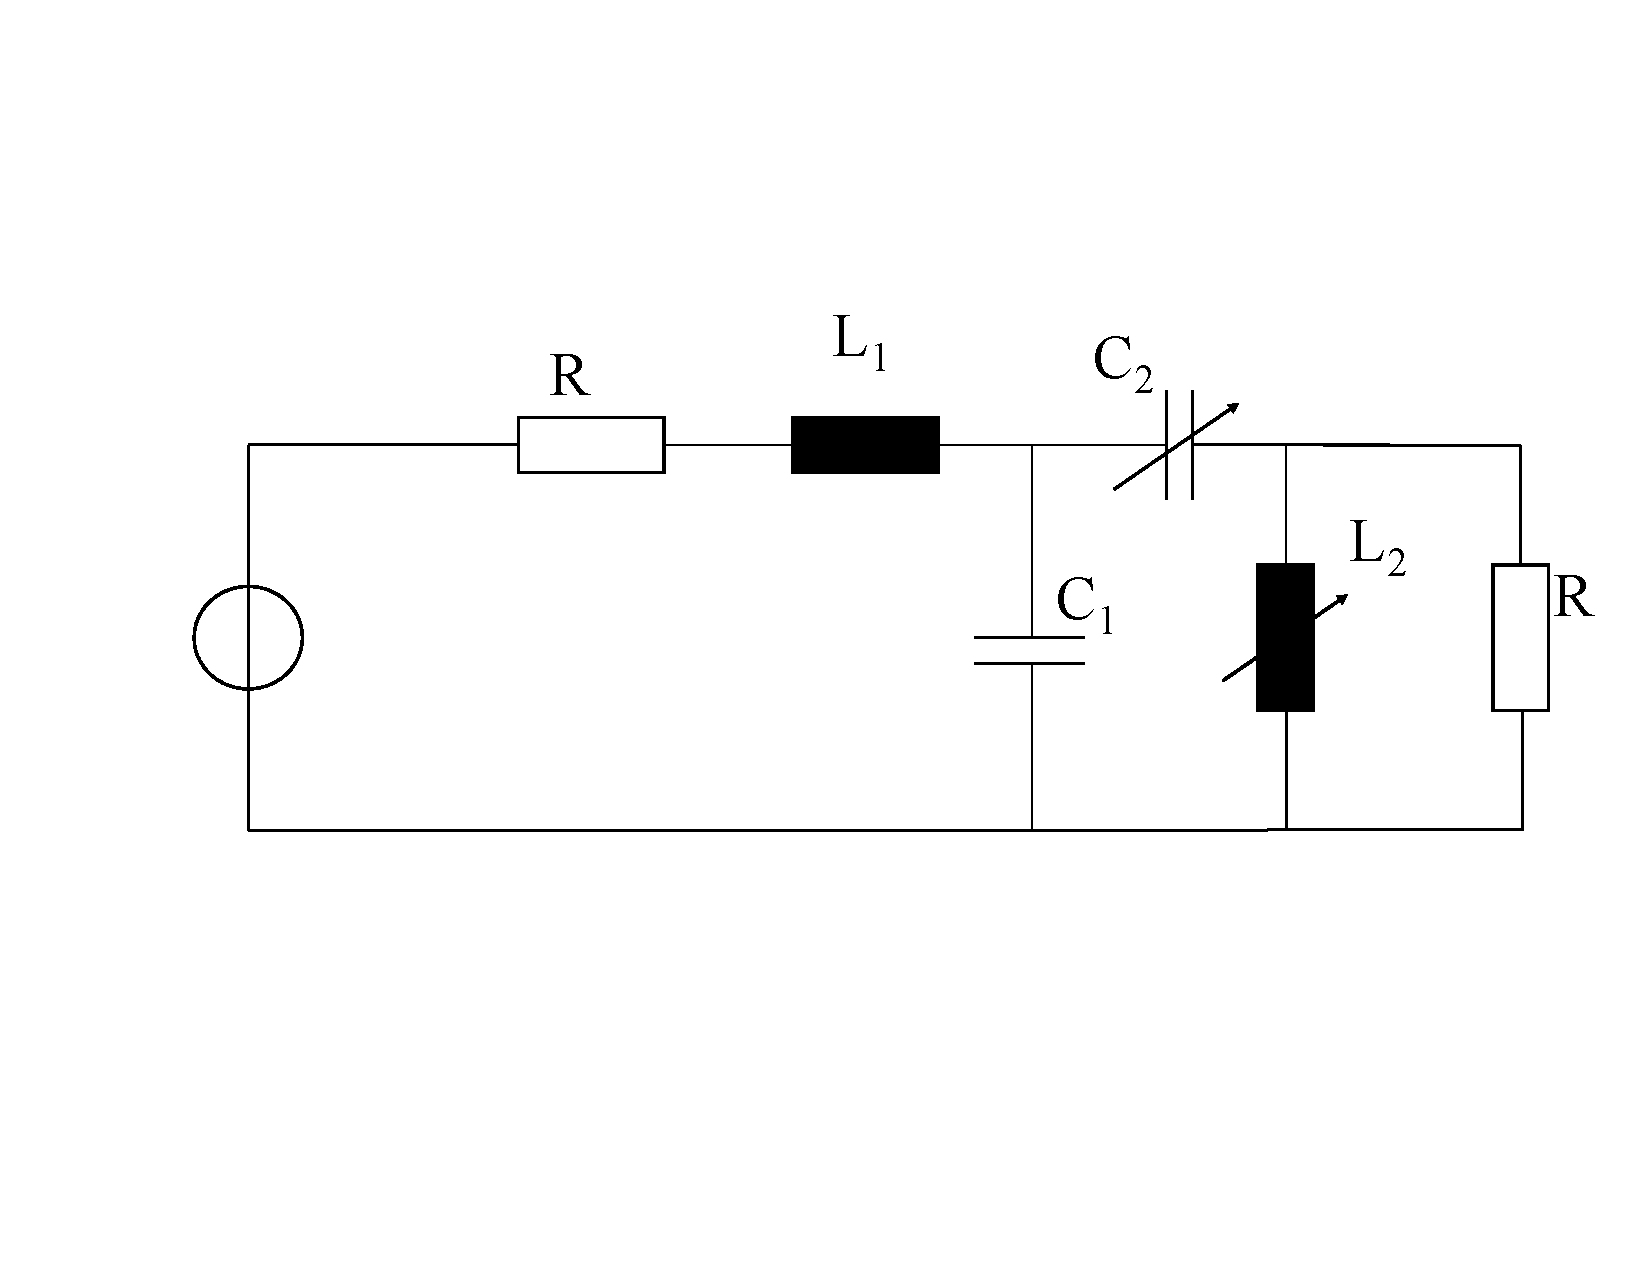
\includegraphics[scale=0.5, trim =1cm 7cm 1cm 5cm,clip ]{linear_filter.pdf}
	\caption{Linear Filter, fixed parameters}
	\label{linearfilter} 
\end{figure}


$C_2$ in graphic \ref{linearfilter} can be tuned $\rightarrow$ programmable filter (due to changeable parameters). Note that this is not an Adaptive Filter yet, just a programmable one.\\
E.g. Bandpass with changeable frequency but same bandwidth (you have to change all: C, R and L!). Changing all parameters would make this filter not fixed. 


Continuous --> Digital --> easier 

\subsection{Digital Filter:}
\begin{figure}[H]
	\centering
	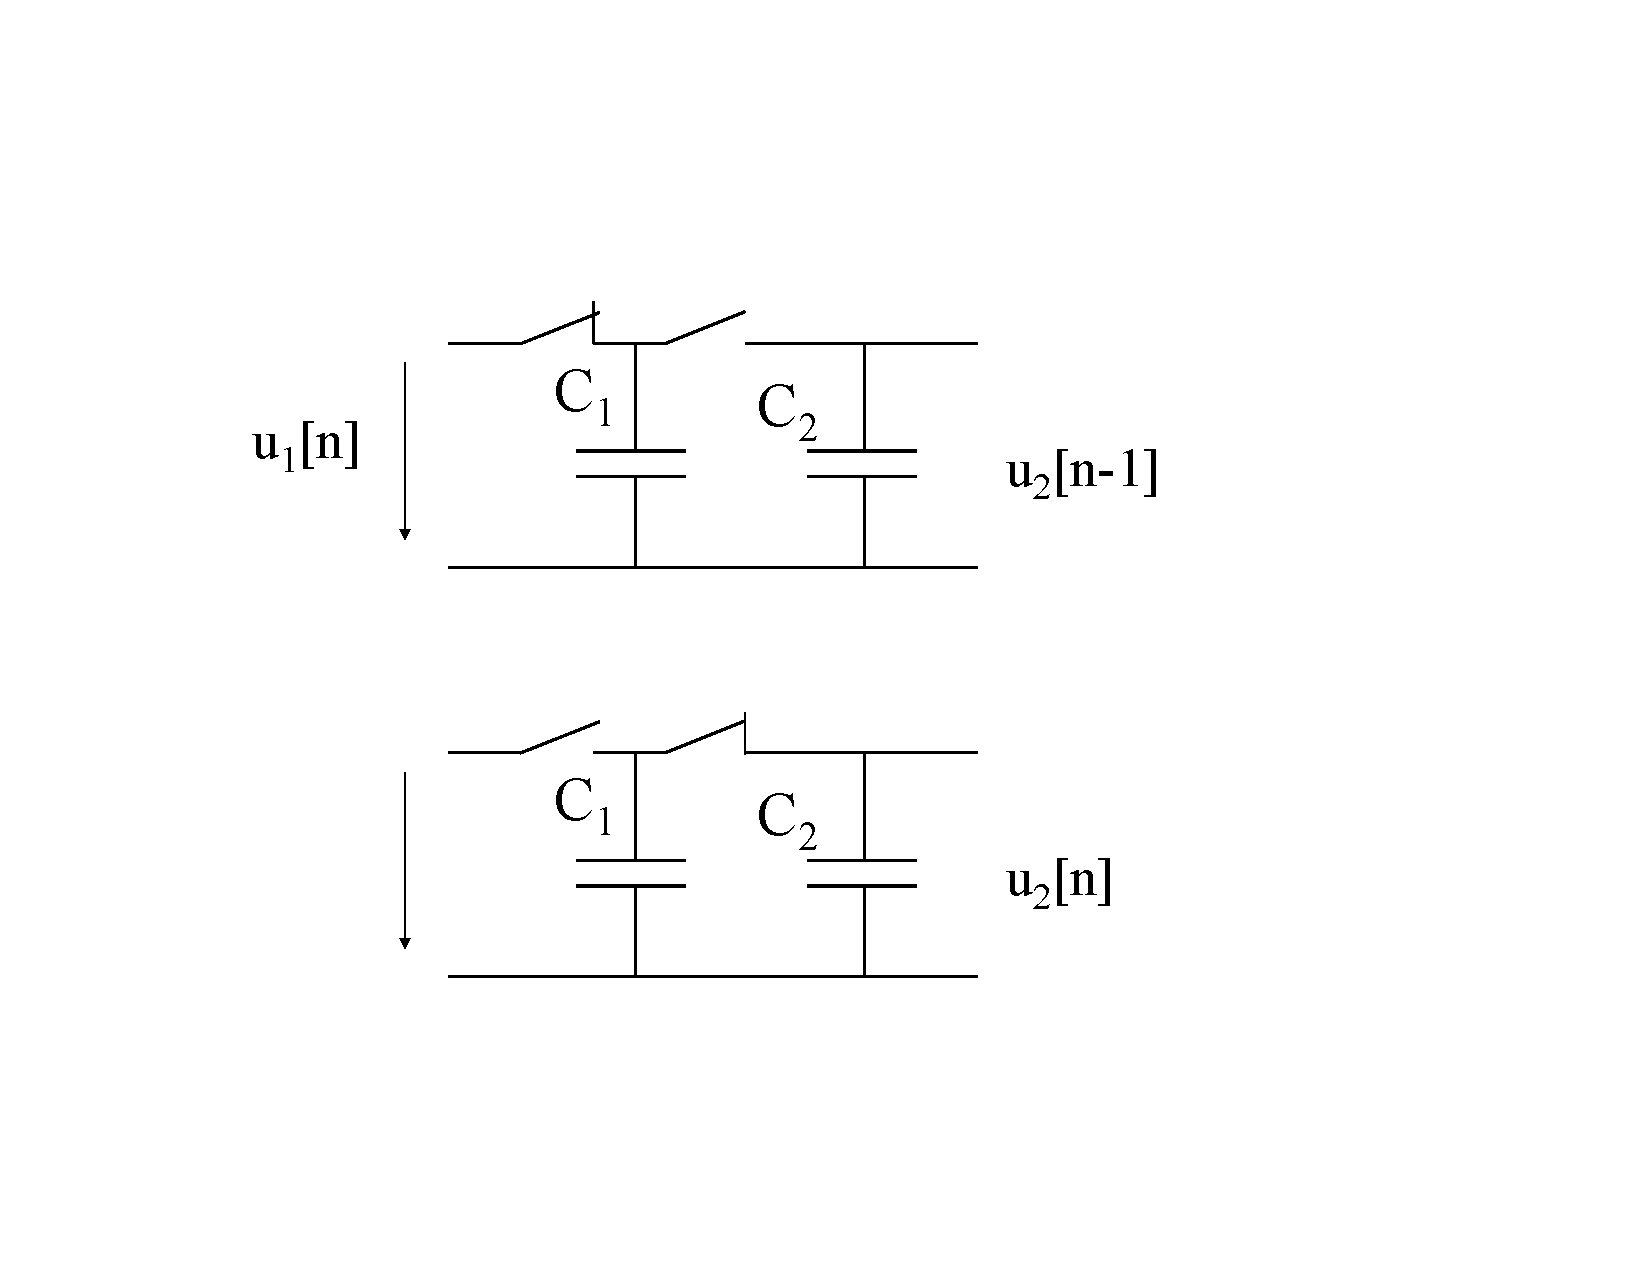
\includegraphics[scale=0.5, trim =3cm 5cm 6cm 5cm,clip ]{discrete_filter.pdf}
	\caption{One open, one closed, discrete time filter}
	\label{discretefilter} 
\end{figure}

Step 1: 	 \\Trans. 1 opened\\
			 Trans. 2 closed\\

Step 2:      \\Trans. 1 closed\\
			 Trans. 2 opened\\

The steps correspond to the discrete clock cycles.


\subsubsection{IIR-Filter}
Infinite impulse response (IIR) is a property applying to many linear time-invariant systems. Common examples of linear time-invariant systems are most electronic and digital filters. Systems with this property are known as IIR systems or IIR filters, and are distinguished by having an impulse response which does not become exactly zero past a certain point, but continues indefinitely. This is in contrast to a finite impulse response (FIR) in which the impulse response h(t) does become exactly zero at times $t > T$ for some finite T, thus being of finite duration.
The discrete filter in picture \ref{discretefilter} is defined by:\\ 
$C_1\cdot u_1[n] + C_2\cdot u_2[n-1] = (C_1+C_2 )u_2[n]$\\ 
$u_2[n]= \underbrace{\frac{C_2}{C_1+C_2}}_{a}\cdot u_2[n-1] + \underbrace{\frac{C_1}{C_1+C_2}}_{1-a}\cdot u_1[n]$\\
It's impulse response is given by table \ref{tab:prog_filter_Impulse_Resp}. As can be seen coefficient $a$ allows us to change the filter's impulse response and therefore to program the filter. Figure \ref{discreteeasy} shows a block diagram for such an easy, programmable discrete filter. From this block diagram it can be seen immediately that this filter is an IIR-Filter and can therefore be unstable.
\begin{figure}[H]
	\centering
	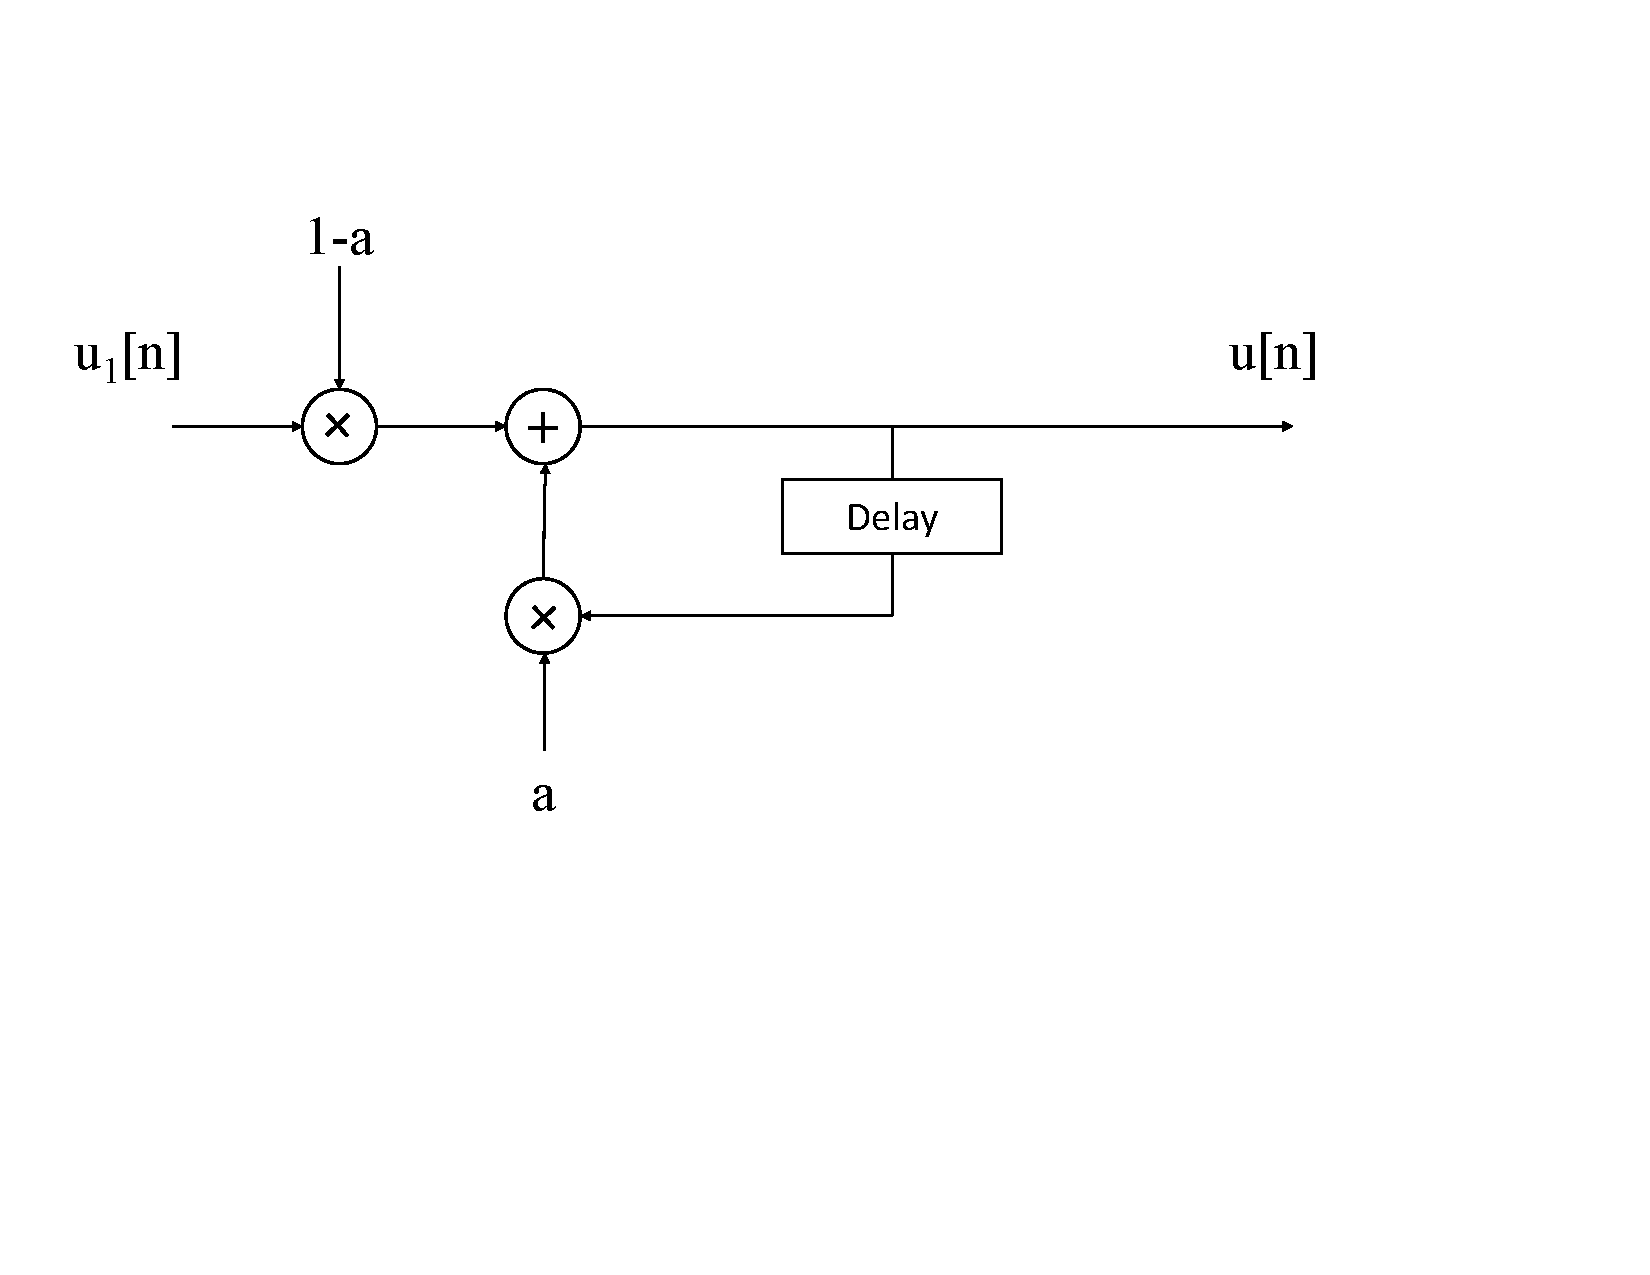
\includegraphics[scale=0.5, trim=1cm 7cm 3cm 2cm,clip]{discrete_easy.pdf}
	\caption{Discrete, easy to software implement filter}
	\label{discreteeasy} 
\end{figure}

\begin{table}
	\caption{discrete filter - Impulse Response }	
	\label{tab:prog_filter_Impulse_Resp}
	\centering
\begin{tabular}[H]{|c|cccccc|}
\hline
	n & $\leq$ 0 & 0 &1 &2 & ... &k\\
	\hline
	$u_1[n]$& 0 & 1 & 0 & 0 & ... &0\\
	$u_2[n]$& 0 & $1-a$ & $a(1-a)$&$ a^2(1-a) $& ... & $a^k (1-a)$\\
	\hline
	\label{wertetabelle}
\end{tabular}
\end{table}

The beauty of going from Analog to Digital is that it opens the option to input anything as $a$, even Complex numbers/variables. 

$\rightarrow$ Stability Issue: 

$y[n]$ = $\sum_{m=-\inf}^{+\inf}h[m]x[n-m]$

digital filters may be 
\begin{itemize} 
	\item bounded $(-\infty, +\infty)$
	\item unstable 
\end{itemize}


$\rightarrow$ we will introduce that 	$x[n] \leq A < \infty$

This is the condition for stability.

which means...\\

$|y[n]| \leq A \sum_{m=-\infty}^{+\infty} | h[m] | < \infty $


In case we have a \textit{Bounded In Bounded Out (\textbf{BIBO})} Filter: 
$x[m] = h^{*}[n-m] / |h[n-m]|$

$\rightarrow$ for BIBO (stable) $|y[n]| = \sum_{m=-\inf}^{+\inf}|h[m]| < \infty$

We can manipulate a in \ref{discreteeasy}. From Table \ref{wertetabelle} we get:

\begin{equation}
 h[n] = \begin{cases}
       (1 - a)^n &  \text{for x $\leq$ 0} \\
       0 & \text{else} \\
     \end{cases}
\end{equation}


\textbf{Stability Requirement:} 
\begin{equation}
\boxed{|a| \leq 1}
\end{equation}

Must be in the unit circle! 

IIR are not used for adaptive Filters


\subsubsection{FIR-Filter}

To overcome the stability problems an FIR-filter can be used instead. FIR-Filters are always stable.
Suitable for adaptive filters but it's an approximation \pfeil finite. Math and informatics can get good aproximations for $\rightarrow \infty$. \\
Structure: tapped delay line \\
linear: neither delay nor coefficient are dependent on input signal. $\rightarrow$ linear adaptive filter, see picture \ref{delayfilter}.\\ \\

\begin{figure}[H]
	\centering
	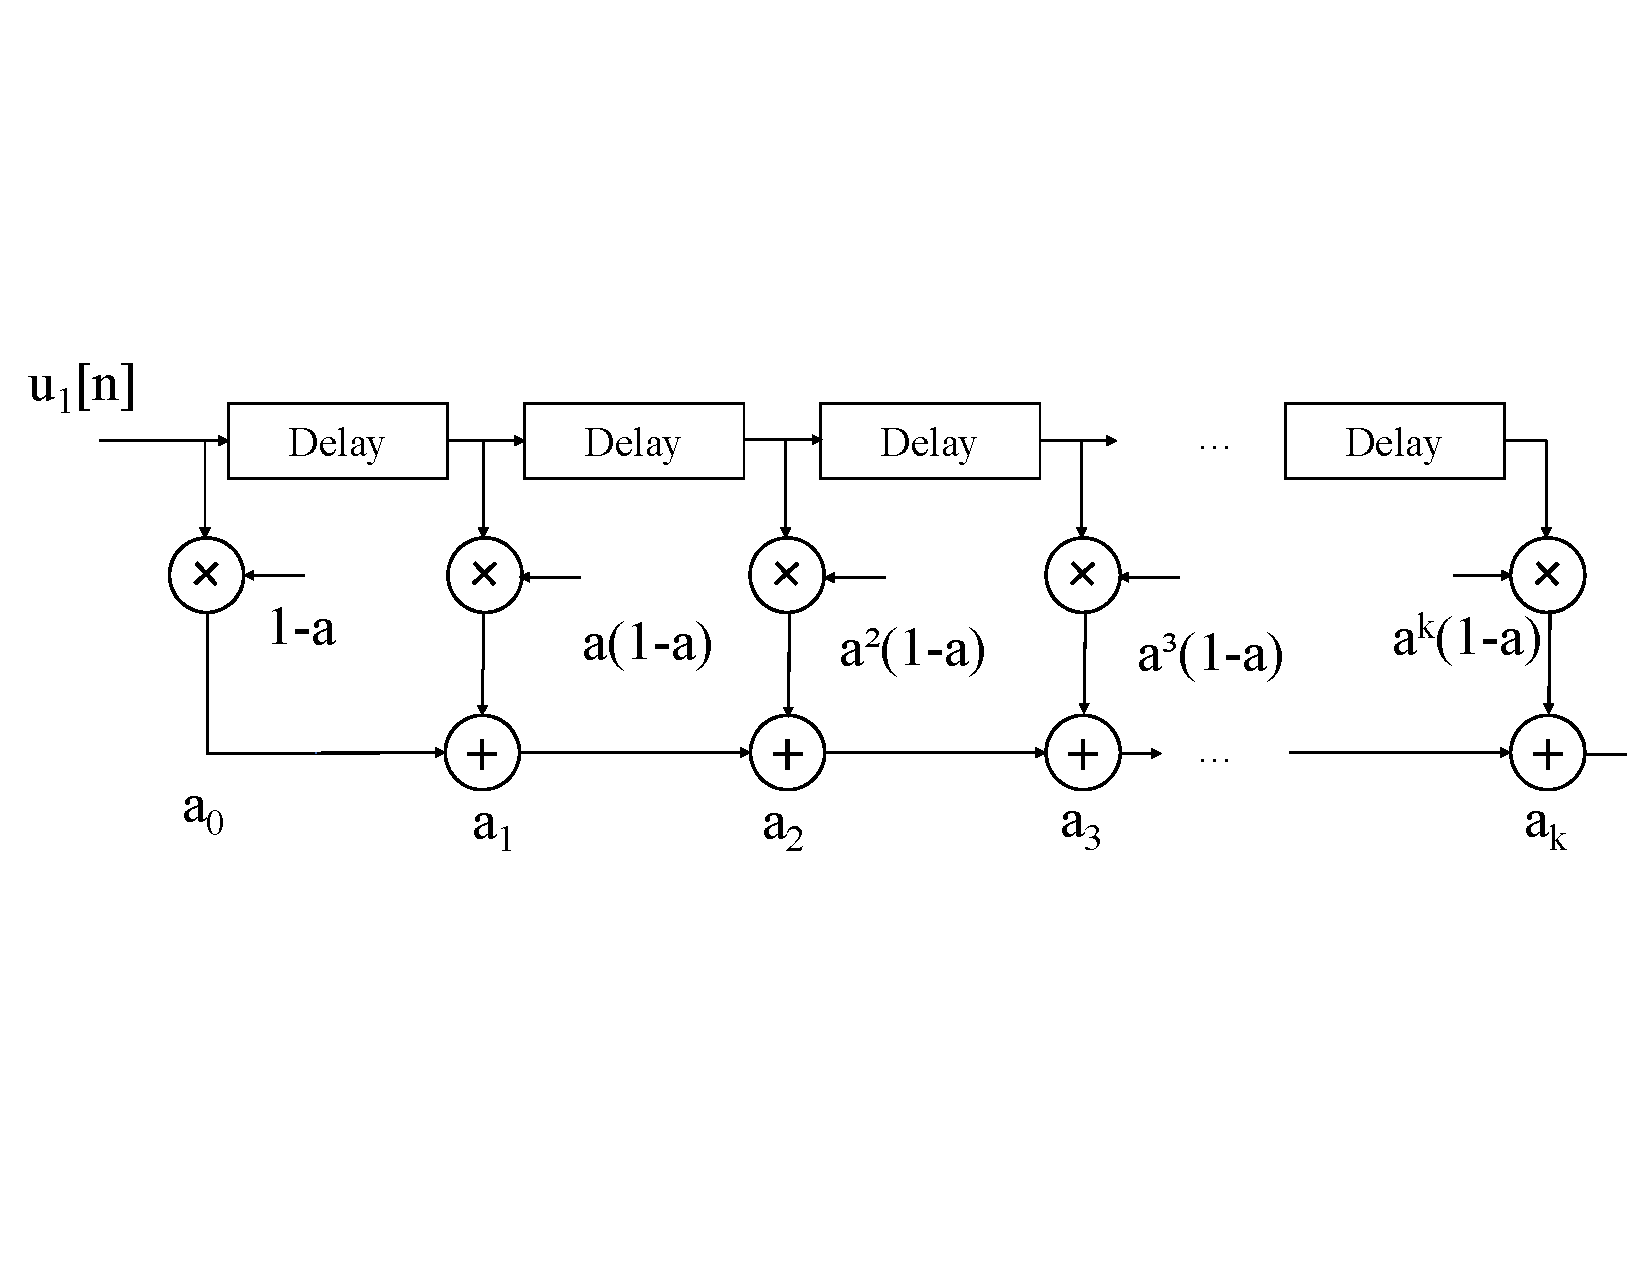
\includegraphics[scale=0.5, trim=0cm 5cm 0cm 5cm,clip]{delay_filter.pdf}
	\caption{Linear adaptive filter (tapped delay line)}
	\label{delayfilter} 
\end{figure}

\textbf{Delays of 1 clock cycle:}\\
$D\cdot x[n] = x[n-1]$\\ \\
\textbf{Delay of 2 clock cycles:}\\
$\underbrace{DD}_{D^2}\cdot x[n] = D \cdot x[n-1] = x[n-2]= D^2\cdot x[n] $\\ \\

\textbf{Fractional delay:}\\
$F \cdot x(n) = x(n-\frac{1}{2})$\\
$FF \cdot x(n) = F \cdot x(n-\frac{1}{2}) = x[n-1] = D \cdot x[n]$\\
$F^2 = FF  	\equiv D ; F= \sqrt{D} = D^{\frac{1}{2}}$\\
$D^{\frac{1}{2}} \cdot D^{\frac{1}{2}} = D^{\frac{1}{2}+\frac{1}{2}} = D' =D$ \\
Developed using a Taylor series: $D^{\frac{1}{2}} \approx  1+\frac{1}{2}(D-1)+ \frac{1}{8}(D-1)^2 = \frac{3}{8}+\frac{3}{4}\cdot D + \frac{1}{8} D^2$\\

\textbf{Second order Taylor expansion $\rightarrow$ Second degree Filter}

The filter in graphic \ref{delayfilter1_2} shows the shifting of the signal by $\frac{1}{2}$.
\begin{figure}[H]
	\centering
	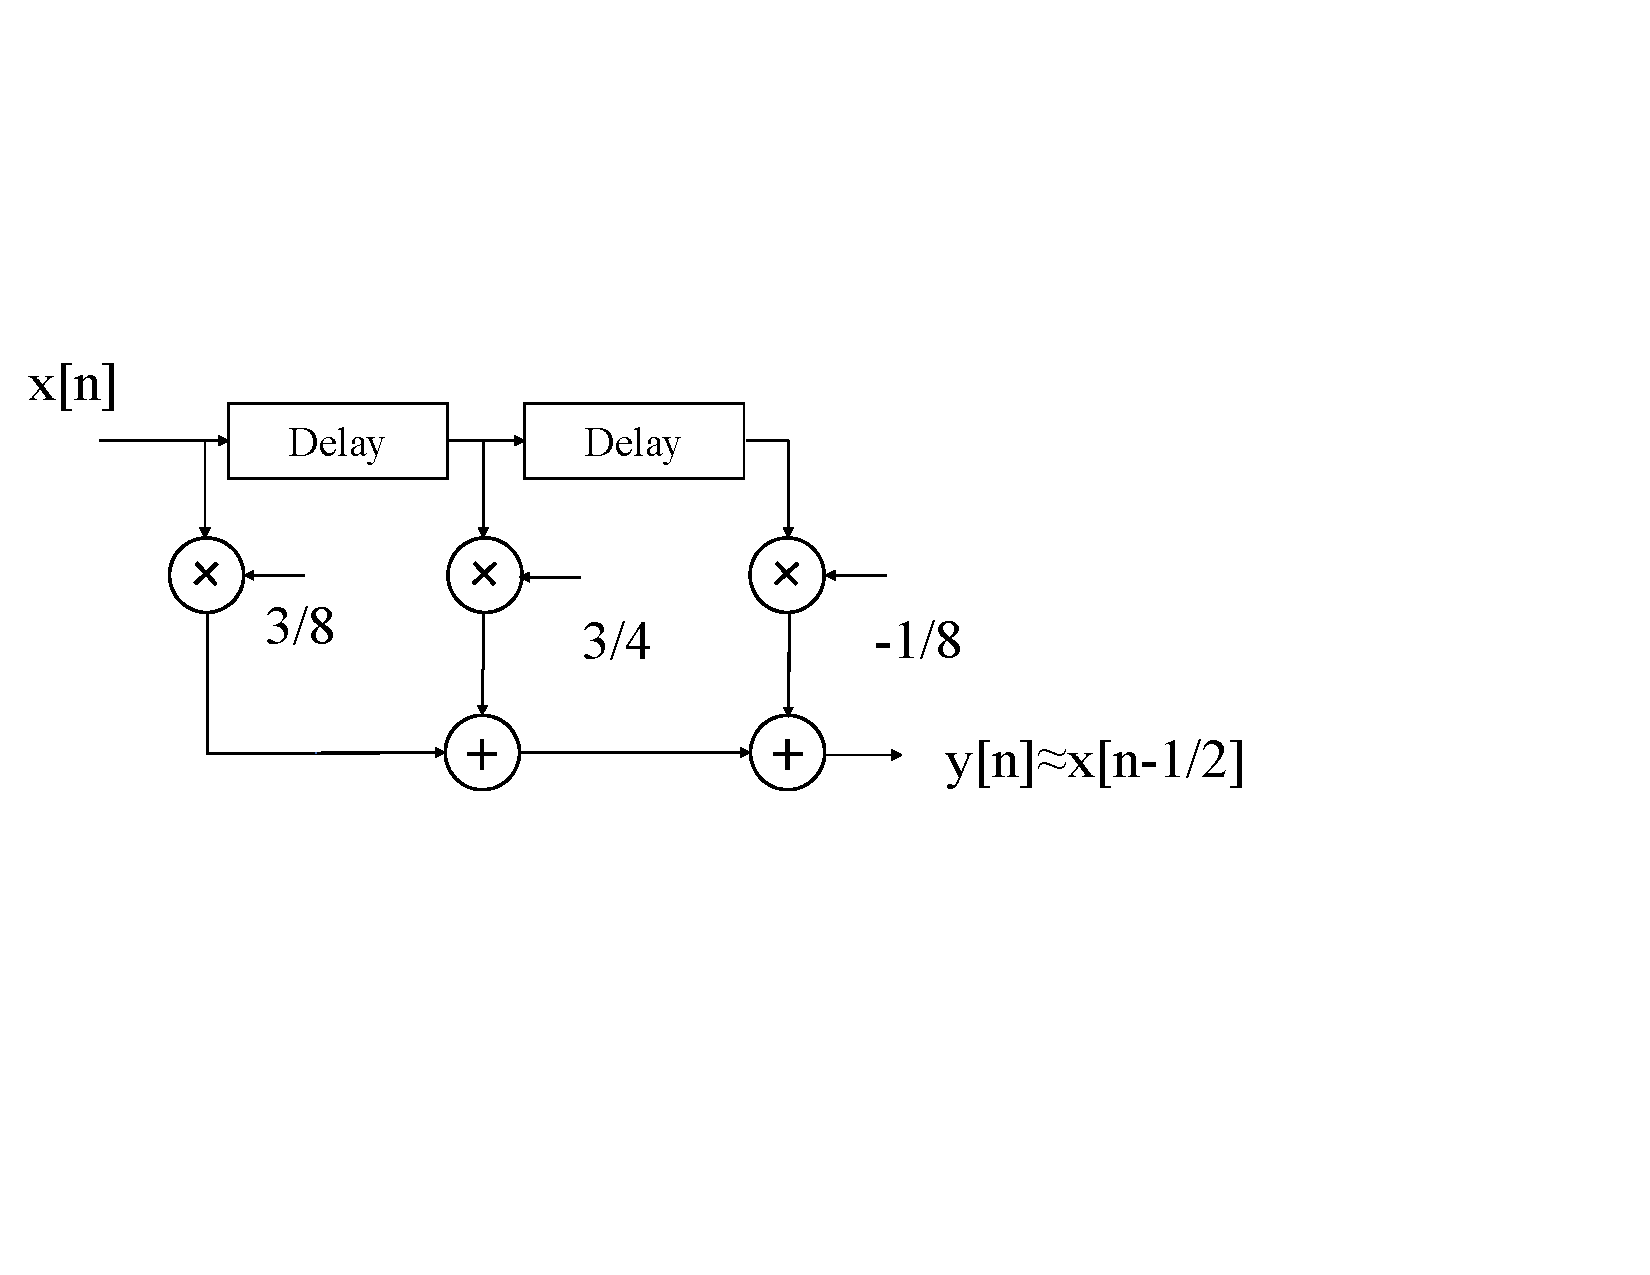
\includegraphics[scale=0.5, trim=0cm 8cm 0cm 6cm, clip]{delay_1_2.pdf}
	\caption{Used for synchronization of receiver and transmitter}
	\label{delayfilter1_2} 
\end{figure}


A fractional delay $y[n] \approx u[n-a] $ for $0 \leq a \leq 1$ \\
$y[n] = a_0 \cdot u[n] + a_1 \cdot u[n-1] + a_2 \cdot u[n-2] $ \\

\begin{itemize} 
	\item $ a_0 = \frac{1}{2} (a^2 - 3a + 2)$ 
	\item $a_1 = (2-a)a$ 
	\item $a_2= \frac{1}{2} (a-1) a $\\
\end{itemize}

\begin{figure}[H]
	\centering
	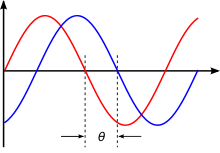
\includegraphics{phaseshift.png}
	\caption{Phase-shift for $\theta$}
	\label{phaseshift} 
\end{figure}

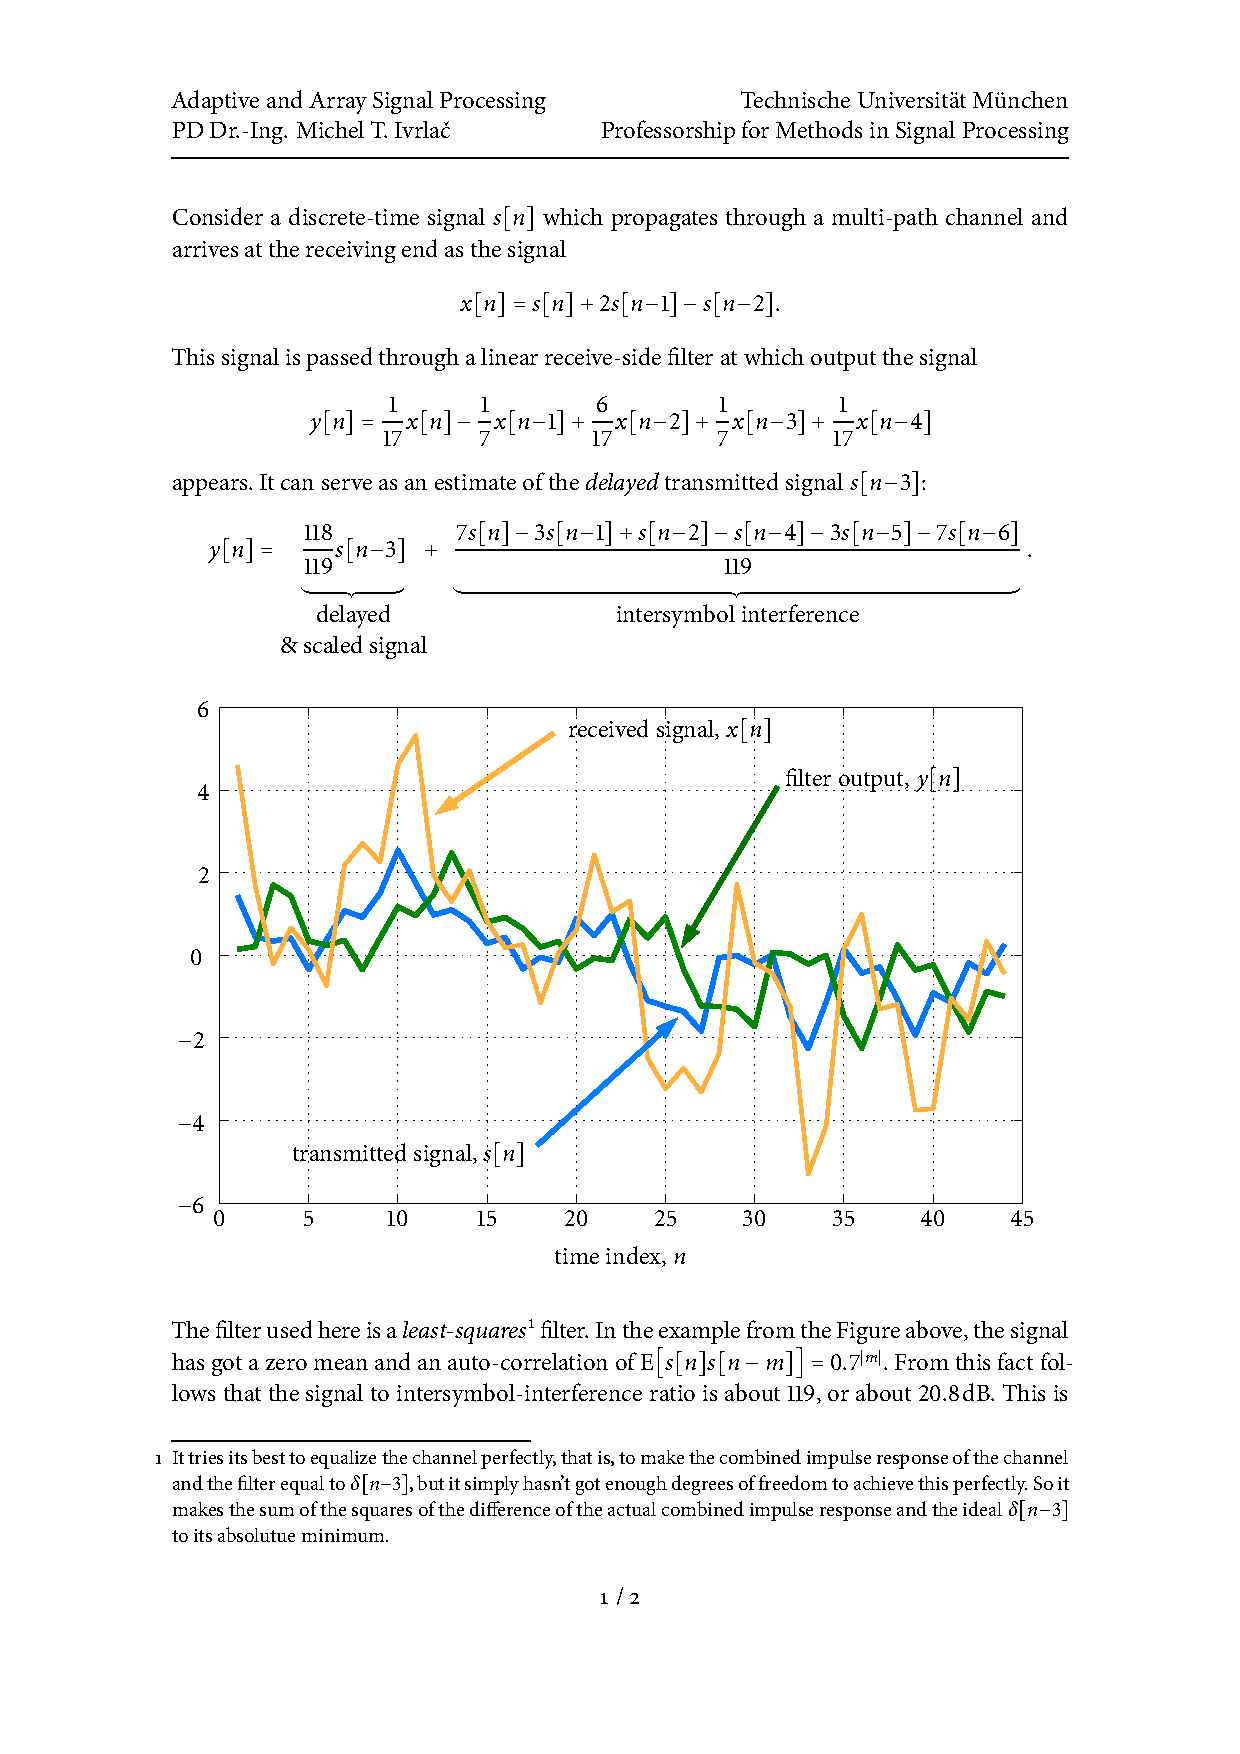
\includepdf[page={1,2}]{pdfs/lect1.pdf}



%\input{AASP_Math_general}
%\input{AASP_Math_derivative}
%\input{AASP_Math_Minimization}
%\input{AASP_Math_Linear_Algebra}
%\input{AASP_Math_Statistics}
%\newpage
%\input{AASP_Optimum_Linear_Filtering}
%\newpage
%\input{AASP_Spartial_Filtering}
%\newpage
%\input{AASP_Estimation_Steering_Matrix}
%\newpage
\printbibliography
\end{document}